% arara: xelatex
% arara: xelatex
% arara: xelatex

% options:
% thesis=B bachelor's thesis
% thesis=M master's thesis
% czech thesis in Czech language
% english thesis in English language
% hidelinks remove color boxes around hyperlinks

\documentclass[thesis=M,english]{FITthesis}[2012/10/20]

\usepackage{graphicx} %graphics files inclusion
% \usepackage{subfig} %subfigures
% \usepackage{amsmath} %advanced maths
% \usepackage{amssymb} %additional math symbols

\usepackage{dirtree} %directory tree visualisation

% list of acronyms
% \usepackage[acronym,nonumberlist,toc,numberedsection=autolabel,nomain]{glossaries}
\iflanguage{czech}{\renewcommand*{\acronymname}{Seznam pou{\v z}it{\' y}ch zkratek}}{}
% \makeglossaries

\newcommand{\tg}{\mathop{\mathrm{tg}}} %cesky tangens
\newcommand{\cotg}{\mathop{\mathrm{cotg}}} %cesky cotangens

% % % % % % % % % % % % % % % % % % % % % % % % % % % % % % % % % % % 
% % % % % % % % % % % % % % % % % % % % % % % % % % % % % % % % % % % 
\department{Department of Applied Mathematics}
\title{Detecting similarities of data domains using machine learning methods}
\authorGN{Andrej Oliver} %author's given name/names
\authorFN{Chud\'y} %author's surname
\authorWithDegrees{Bc. Andrej Oliver Chud\'y} %author's name with academic degrees
\author{Andrej Oliver Chud\'y} %author's name without academic degrees
\supervisor{Ing. Zdenek Buk, Ph.D.}
\acknowledgements{I would like to thank my family and friends for support during writing this thesis.}
\abstractCS{
% TODO
}
\abstractEN{
% TODO
}
\placeForDeclarationOfAuthenticity{Prague} %where you have signed the declaration
\keywordsCS{}
\keywordsEN{Natural Language Processing, Deep learning, NLP, RNN, CNN, embedding, LSTM, GRU.}
\declarationOfAuthenticityOption{4} %select as appropriate, according to the desired license
\website{http://site.example/thesis} %optional URL (remove entirely if you have no URL for this thesis)

\begin{document}


\begin{introduction}

	\section{Objectives}

	\section{Challenges}

\end{introduction}

\chapter{Preliminaries}

\section{What is Deep Learning?}
First, we need to define clearly what we're talking about. What deep learning is? Deep learning is a specific subfield of machine learning. The deep in deep learning isn't a reference to any kind of deeper understanding but it stands for the idea of successive layers of representations. The count of layers contribute to a model called the depth of the model. Modern deep learning often involves tens or even hundreds of successive layers of representations and they've all learned automatically from exposure training data. In deep learning, these layered representations are (almost always) learned via models called neural networks, structured in literal layers stacked on top of each other. On the next image, you can see how a network several layers deep look like.


\begin{figure}\centering
	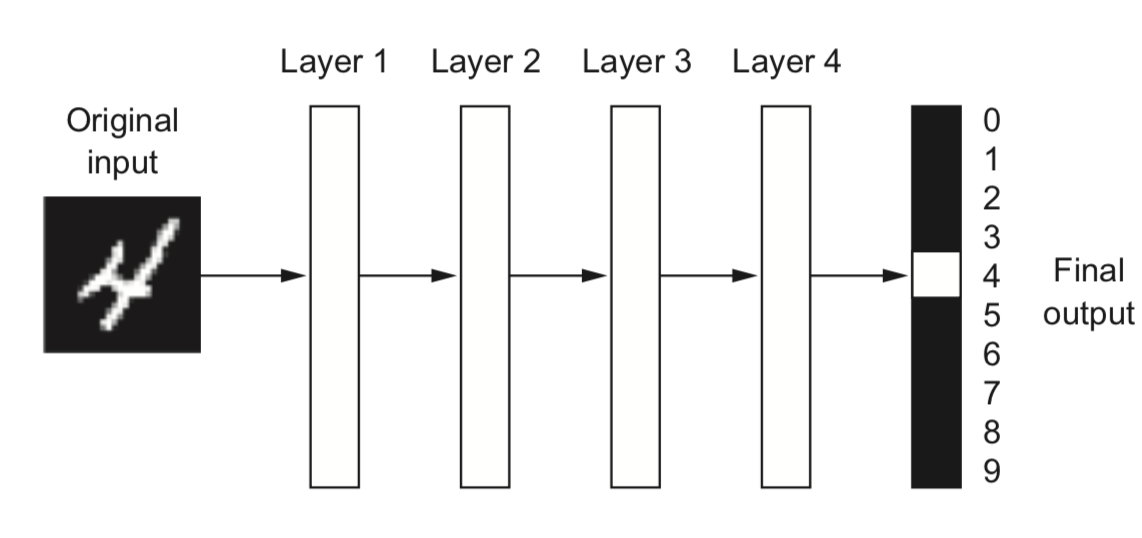
\includegraphics[scale=0.6]{images/deep_NN}
	\caption{Deep neural network}\label{fig:deep NN}
\end{figure}

\subsection{Training of neural networks}
The learning process in a neural network is about mapping inputs (image, text, or something else) to target (some label such as category or continues value) via a deep sequence of simple transformations (layers) and that these data transformations are learned by exposure to examples. 

The specification of what a layer does to its input data is stored in the layer's weights, which in essence are a bunch of numbers. In technical terms, we'd say that the transformation implemented by a layer is parameterized by its weights. In this context, learning means finding a set of values for the weights of all layers in a network, such that the network will correctly map example inputs to their associated targets. But a deep neural network can contain tens of millions of parameters. Finding the correct values for all of them is a very hard optimization task. 

To judge the output of a neural network, you need to be able to measure how far this output is from what you expected. This is the job of the \textbf{loss function} of the network. The \textbf{loss function} takes the predictions of the network and the true target and computes a distance score, capturing how well the network has done on this specific example. The fundamental trick in deep learning is to use this score as a feedback signal to adjust the value of the weights a little, in a direction that will lower the loss score for the current example. This adjustment is the job of the \textbf{optimizer}, which implements what's called the \textbf{Backpropagation} algorithm which is the most famous algorithm in machine learning for optimization of hyperparametric space of NN.


\section{Recurrent neural networks}
A principal of the work of the recurrent neural network is more similar to the human brain. When humans read the text, they understand each word based on the understanding of previous words. Traditional feed-forward neural networks can't do this. Recurrent neural network address this problem. Those networks contain loops, allowing persist information.
















\section{Convolution neural networks (CNN)}
\section{Recurrent neural networks (RNN)}
\section{LSTMs}
\section{Summary}




\chapter{Implementation and testing}\label{impltest}

\section{Details of realised tests}


\section{Integers distribution and encoding}\label{sec:distr}

The integers encoding of indexes of phrases from the word (non-word) dictionary is possible cause of the only average results of compression ratio of implemented algorithms. The decision is to get the distribution of indexes during the encoding process (and decoding process too). The length of indexes located in shown graphs is only hypothetical---the binary code with minimal length.

The graphs of index distribution also shows the differencies between the algorithms with sorted dictionaries (\textit{WLZWS} and \textit{WLZWES}) and the algorithms with unsorted dictionaries (\textit{WLZW} and \textit{WLZWE}). The most frequently used phrases are moved to the front of dictionary in algorithms with sorted dictionary so they get lower indexes. This feature is demonstrated by the growth of number of indexes at the beginning of the distribution. The compression process of algorithms with sorted dictionaries becomes more efficient when the code with variable length of code words (Fibonacci code) is used but the compression efficiency is supposed to be the same at the transition from the \textit{WLZWE2} algorithm to the \textit{WLZWES2} algorithm---the encoding by block code. 

\begin{conclusion}
	The word-based dictionary data compression algorithms (a part of lossless data compression) are the subject of this thesis. The lossless data compression is a very important field of research because the data compression allows to reduce the amount of space needed to store data.

	The background of data compression field was presented in Chapter~\ref{textcompr}. There are basic notions and definitions followed by description of character-based dictionary algorithms. The word-based dictionary compression methods were investigated and discussed at the end of this chapter too.

% 	There is the investigation of index distribution of tested files in Section \ref{sec:distr}. It led to the new modification of semi-adaptive word-based \gls{LZW} algorithm---\textit{WLZWE2}. The compression efficiency of this algorithm applied to the large files is better than the other implemented algorithms. However, the compression efficiency of \textit{WLZWE2} algorithm is much worse when it is applied to the small files. The experiments with \textit{WLZWE2} and \textit{WLZWES2} algorithms confirm the assumption from Section \ref{sec:distr}---the compression efficiency of version with unsorted dictionaries (\textit{WLZWE2}) is analogous to version with sorted ones (\textit{WLZWES2}).

	The testing of memory used during compression and/or decompression process is one of the possibilities of further research. The experiments with files of greater size or multilingual files could be also good opportunity to gain new improvements of algorithms. The static part of dictionaries could improve the compression efficiency too.

	The implemented methods achieve fairly good compression ratio (25--30$\%$ at large files) with acceptable compression and decompression time. There are possibilities of further improvements especially at semi-adaptive methods. However, the gain of these improvements is not good enough to top the compression efficiency of other lossless data compression methods (context methods from PPM family). The results of implemented algorithms were not as good as it was expected but the work on this thesis showed new ways of possible further research---word-based version of grammar-based compression algorithms and another possibilities in the field of word-based context methods of data compression.

	The Gnuplot 4.2 utility was very useful for generation of graphs in this thesis. There was the drawing editor Ipe 6.0 used for figures creation.
	\nocite{Po01}
\end{conclusion}

\bibliographystyle{iso690.bst}
\bibliography{ref}

\appendix

% \printglossaries

\chapter{Contents of CD}\label{app:CDcontent}

Visualise the contents of enclosed media. Use of \verb|dirtree| is recommended. Note that directories src and text with appropriate contents are mandatory.


\begin{figure}
	\dirtree{%
		.1 readme.txt\DTcomment{the file with CD contents description}.
		.1 data\DTcomment{the data files directory}.
		.2 graphs\DTcomment{the directory of graphs of experiments}.
		.3 *.eps\DTcomment{the B/W graphs}.
		.3 *.png\DTcomment{the color graphs}.
		.3 *.dat\DTcomment{the graphs data files}.
		.1 exe\DTcomment{the directory with executable WBDCM program}.
		.2 wbdcm\DTcomment{the WBDCM program executable (UNIX)}.
		.2 wbdcm.exe\DTcomment{the WBDCM program executable (Windows)}.
		.1 src\DTcomment{the directory of source codes}.
		.2 wbdcm\DTcomment{the directory of WBDCM program}.
		.3 Makefile\DTcomment{the makefile of WBDCM program (UNIX)}.
		.2 thesis\DTcomment{the directory of \LaTeX{} source codes of the thesis}.
		.3 figures\DTcomment{the thesis figures directory}.
		.3 *.tex\DTcomment{the \LaTeX{} source code files of the thesis}.
		.1 text\DTcomment{the thesis text directory}.
		.2 thesis.pdf\DTcomment{the Diploma thesis in PDF format}.
		.2 thesis.ps\DTcomment{the Diploma thesis in PS format}.
	}
\end{figure}


\end{document}
